\chapter{Experimentelle Bestätigung des Photons}
\setcounter{section}{4}
\setcounter{subsection}{0}
\setcounter{subsubsection}{1}
\setcounter{secnumdepth}{3}
\setlength{\parindent}{0pt}
% Boxen-Stile definieren
\tcbset{physikbox/.style={colback=blue!5!white, colframe=blue!75!black, fonttitle=\bfseries}}
\tcbset{mathebox/.style={colback=green!5!white, colframe=green!50!black, fonttitle=\bfseries}}
\tcbset{didaktikbox/.style={colback=yellow!5!white, colframe=yellow!50!black, fonttitle=\bfseries}}
\tcbset{hypobox/.style={colback=orange!5!white, colframe=orange!75!black, fonttitle=\bfseries}}
\tcbset{hinweisbox/.style={colback=gray!10!white, colframe=black!40!black, fonttitle=\bfseries}}
\subsection{Der Photoeffekt }\index{Photoeffekt}

\subsubsection{ Einleitung und klassische Erwartung}\index{Klassische Elektrodynamik}\index{Wellenmodell}

Der sogenannte Photoeffekt – die Emission von Elektronen aus einer Metalloberfläche durch Bestrahlung mit Licht – war bereits im 19. Jahrhundert bekannt. Heinrich Hertz\index{Hertz, Heinrich} entdeckte das Phänomen 1887 zufällig bei seinen Untersuchungen zur elektromagnetischen Wellenstrahlung. Philipp Lenard\index{Lenard, Philipp} untersuchte es später systematisch und stellte fest: Es werden Elektronen aus dem Metall gelöst, wenn Licht einer bestimmten Art darauf trifft.

Die klassische Elektrodynamik erklärte dieses Verhalten mit Hilfe des Wellenmodells des Lichts\index{Wellenmodell}. Demnach sollte die Energie des Lichts kontinuierlich über die elektrische Feldstärke an das Elektron übertragen werden. Daraus folgten drei scheinbar plausible Erwartungen:

\begin{itemize}
	\item \textbf{Intensität entscheidet:} Je stärker die Lichtintensität, desto energiereicher müssten die ausgelösten Elektronen sein.
	\item \textbf{Verzögerung:} Bei schwachem Licht müsste eine messbare Zeit vergehen, bis ein Elektron genügend Energie aufgenommen hat, um emittiert zu werden.
	\item \textbf{Jeder Wellenlänge möglich:} Prinzipiell müsste jede Wellenlänge Licht – auch langwelliges rotes – zur Elektronenemission führen, wenn es nur intensiv genug ist.
\end{itemize}

Diese Erwartungen schienen logisch im Rahmen der klassischen Theorie. Doch sie wurden von der Realität drastisch widerlegt – ein Wendepunkt in der Geschichte der Physik.

\vspace{1em}
\begin{tcolorbox}[physikbox, title=Philipp Lenard (1902)\textit{ \cite{lenard1902} }]
	\label{box:Philipp Lenhard}
	\small
	„Es zeigte sich, dass das Licht mit größerer Energie auf die Elektronen zu wirken schien,\\
	je kürzer seine Wellenlänge war – ganz unabhängig davon, wie hell es war.“
\end{tcolorbox}

\subsubsection{Experimentelle Beobachtungen}

Die systematische Untersuchung des Photoeffekts durch Philipp Lenard\index{Lenard, Philipp}, Robert Millikan\index{Millikan, Robert A.} und andere führte zu Beobachtungen, die sich mit der klassischen Wellentheorie nicht vereinbaren ließen. Die zentralen experimentellen Befunde lauten:

\begin{itemize}
	\item \textbf{Sofortige Emission:} Die Elektronen werden ohne messbare Verzögerung freigesetzt – selbst bei extrem schwacher Lichtintensität.
	\item \textbf{Frequenzabhängigkeit:} Es existiert eine \emph{Grenzfrequenz} \( \nu_{\text{min}} \)\index{Grenzfrequenz}, unterhalb der keine Elektronen ausgelöst werden – unabhängig von der Intensität.
	\item \textbf{Intensitätsunabhängigkeit der Energie:} Die kinetische Energie der ausgelösten Elektronen hängt ausschließlich von der Frequenz des Lichts ab – nicht von seiner Intensität.
	\item \textbf{Linearer Zusammenhang:} Die Elektronenenergie steigt linear mit der Lichtfrequenz:
	\[
	E_{\text{kin}} = h \nu - A
	\]
	\index{Einstein-Gleichung (Photoeffekt)@Einstein-Gleichung (Photoeffekt)}\index{Austrittsarbeit}
\end{itemize}
(Eine ausführlichere Herleitung der Einstein-Gleichung für den Photoeffekt findet sich in Anhang~A, Abschnitt~\ref{anhangA:photoeffekt}.)

Diese Ergebnisse widersprachen fundamental der klassischen Erwartung einer kontinuierlichen Energieaufnahme aus dem elektromagnetischen Feld.

\vspace{1em}
\begin{tcolorbox}[physikbox, title=Albert Einstein (1905)\textit{ \cite{einstein1905}} ]
	\label{die Erzeuguung von Licht}
	\small
	„Die Erzeugung von Licht erfolgt nicht überall auf der Wellenfront gleichmäßig, sondern nur an bestimmten Orten, an einzelnen Punkten.“
\end{tcolorbox}
\index{Einstein, Albert}

\vspace{1em}
\begin{tcolorbox}[physikbox, title=Robert A. Millikan (1916)\textit{ \cite{millikan1916}}]
	\label{box:Robert A, Millikan}
	\small
	„Obwohl ich Einsteins Gleichung durch jahrelange Experimente bestätigt habe, konnte ich mich lange nicht mit dem Gedanken anfreunden, dass Licht aus Teilchen besteht.“
\end{tcolorbox}
\vspace{1em}
\index{Millikan, Robert A.}

\textbf{Fazit:} Die Beobachtungen ließen sich nur durch die Annahme erklären, dass Licht aus diskreten Quanten besteht – \emph{Photonen}\index{Photon}\index{Lichtquant|see{Photon}} –, die ihre Energie in einem Stoßprozess an ein Elektron übertragen. Die klassische Wellenvorstellung musste aufgegeben oder tiefgreifend ergänzt werden.
\subsubsection{Einsteins Erklärung (1905)}\index{Einstein, Albert}\index{Lichtquant|see{Photon}}\index{Photon}\index{Heuristischer Gesichtspunkt (Einstein 1905)}

Im Jahr 1905 veröffentlichte Albert Einstein seine bahnbrechende Arbeit mit dem Titel \textit{„Über einen die Erzeugung und Verwandlung des Lichtes betreffenden heuristischen Gesichtspunkt“} \cite{einstein1905}. Darin stellte er die klassische Vorstellung von Licht als kontinuierlicher Welle grundlegend infrage.\index{Klassische Elektrodynamik}\index{Wellenmodell}

Einstein schlug vor, dass Licht aus einzelnen Energieportionen – sogenannten \textbf{Lichtquanten}\index{Lichtquant|see{Photon}} – besteht. Diese Quanten tragen eine bestimmte Energiemenge:

\[
E = h \nu
\]\index{Planck-Einstein-Beziehung@$E=h\nu$}
(Eine formale Darstellung der Planck–Einstein-Beziehung findet sich in Anhang~A, Abschnitt~\ref{anhangA:planckEinstein}.)

Ein Photon mit Frequenz \( \nu \) besitzt also eine diskrete Energie, proportional zur Frequenz. Diese Idee war revolutionär, denn sie sprach dem Licht einen \emph{Teilchencharakter} zu – entgegen der etablierten Wellenvorstellung der Maxwell-Theorie.\index{Maxwell, James Clerk}\index{Maxwell-Theorie@Maxwell-Theorie}

Einstein postulierte weiter, dass ein solches Lichtquant seine Energie in einem Stoßprozess vollständig auf ein Elektron übertragen könne. 

Nur wenn die Energie des Photons größer ist als die sogenannte \textbf{Austrittsarbeit} \( A \), wird ein Elektron aus dem Metall ausgelöst:\index{Austrittsarbeit}

\[
E_{\text{kin}} = h \nu - A
\]\index{Einstein-Gleichung (Photoeffekt)@Einstein-Gleichung (Photoeffekt)}

Diese Gleichung erklärt unmittelbar:
\begin{itemize}
	\item Warum nur Licht mit ausreichend hoher Frequenz Elektronen auslösen kann,
	\item Warum die Emission sofort erfolgt (ein einzelnes Photon genügt),
	\item Warum die kinetische Energie der Elektronen linear mit der Frequenz wächst.
\end{itemize}

Einsteins Erklärung war radikal – und zunächst sehr umstritten. Selbst Max Planck, der Begründer der Quantentheorie, betrachtete die Lichtquantenhypothese als zu spekulativ.\index{Planck, Max}

\vspace{1em}
\begin{tcolorbox}[physikbox, title=Albert Einstein (1905)\textit{ \cite{einstein1905}} ]
	\label{die Erscheinung der Wärm}
	\small
	„Die Erscheinungen der Wärmestrahlung fordern eine Betrachtungsweise, wonach das Licht in der Ausbreitungsrichtung aus diskreten Energiequanten besteht.“
\end{tcolorbox}
\index{Einstein, Albert}
\vspace{1em}
\textbf{Einordnung:} Einstein machte aus Plancks mathematischem Kunstgriff eine physikalische Realität. Damit legte er den Grundstein für den modernen Photonbegriff und die Quantennatur des elektromagnetischen Feldes.\index{Photon}\index{Quantenelektromagnetisches Feld@Quantennatur des elektromagnetischen Feldes}

\subsubsection{Millikans Messungen (1916)}\index{Millikan, Robert A.}

Obwohl Albert Einsteins Lichtquantenhypothese eine überzeugende Erklärung für den Photoeffekt lieferte, blieb sie zunächst heftig umstritten. Viele Physiker – darunter auch Max Planck – hielten es für unvorstellbar, dass Licht aus echten Teilchen bestehen sollte.\index{Planck, Max} Einer der prominentesten Skeptiker war \textbf{Robert A. Millikan}.\index{Millikan, Robert A.}

In einer mehrjährigen Versuchsreihe (1909–1916) entwickelte Millikan ein besonders präzises Experiment, um Einsteins Gleichung systematisch zu überprüfen. Mit Hilfe einer Vakuum-Fotozelle\index{Vakuum-Fotozelle}, exakt justierbarer Gegenspannungen\index{Gegenspannung} und monochromatischer Lichtquellen\index{Monochromatisches Licht} konnte er die maximale kinetische Energie der Elektronen bei verschiedenen Lichtfrequenzen direkt messen.

\textbf{Das Ergebnis:} Millikan fand – trotz aller Zweifel – eine glasklare Bestätigung von Einsteins Vorhersage:

\[
e U = h \nu - A
\]\index{Einstein-Gleichung (Photoeffekt)@Einstein-Gleichung (Photoeffekt)}\index{Austrittsarbeit}
(Eine detaillierte Ableitung der Stoppspannungsgleichung und ihr experimenteller Bezug finden sich in Anhang~A, Abschnitt~\ref{anhangA:stoppspannung}.)

Dabei ist \( U \) die notwendige Gegenspannung zur vollständigen Unterdrückung des Elektronenstroms. Die Steigung der resultierenden Geraden (Elektronenenergie vs. Frequenz) ergab mit hoher Genauigkeit das Plancksche Wirkungsquantum \( h \).\index{Plancksches Wirkungsquantum@$h$ (Plancksches Wirkungsquantum)}

\vspace{1em}
\begin{tcolorbox}[physikbox, title=Robert A. Millikan (1916)\textit{ \cite{millikan1916}} ]
	\label{box:einsteins gleichung passt}
	\small
	„Einsteins Gleichung passt mit erstaunlicher Genauigkeit zu den Daten – und dennoch kann ich mich nicht dazu durchringen, sie als theoretisch befriedigend zu betrachten.“
\end{tcolorbox}
\index{Millikan, Robert A.}
\vspace{1em}
\textbf{Bemerkenswert:} Millikan widerlegte mit höchster Präzision die klassische Theorie – und bestätigte Einsteins Lichtquant – wollte dessen Konzept aber zunächst nicht anerkennen. Erst Jahre später akzeptierte er die quantisierte Natur des Lichts als physikalische Realität.

\textbf{Bedeutung:} Die Messungen von Millikan gelten als einer der wichtigsten experimentellen Nachweise für den Photonenbegriff.\index{Photon} Sie stärkten die Akzeptanz von Einsteins Theorie – auch wenn diese erst mit der Entwicklung der Quantenmechanik umfassend gewürdigt wurde.\index{Quantenmechanik}

\subsubsection{Mathematische Beschreibung}\index{Einstein-Gleichung (Photoeffekt)@Einstein-Gleichung (Photoeffekt)}\index{Austrittsarbeit}

Die zentrale Formel zur Beschreibung des Photoeffekts basiert auf Einsteins Annahme, dass jedes Photon eine diskrete Energie \( E = h\nu \) besitzt.\index{Planck-Einstein-Beziehung@$E=h\nu$} Trifft ein solches Photon auf ein Elektron im Metall, wird seine Energie auf das Elektron übertragen. Dabei gilt die Energiebilanz:

\[
E_{\text{Photon}} = E_{\text{Austritt}} + E_{\text{kin}}
\quad\Rightarrow\quad h \nu = A + E_{\text{kin}}
\]\index{Einstein-Gleichung (Photoeffekt)@Einstein-Gleichung (Photoeffekt)}
\newpage
\noindent
Hierbei ist:

- \( h \) das Plancksche Wirkungsquantum\index{Plancksches Wirkungsquantum@$h$ (Plancksches Wirkungsquantum)}  
- \( \nu \) die Frequenz des einfallenden Lichts\index{Frequenz}  
- \( A \) die materialabhängige \textbf{Austrittsarbeit}\index{Austrittsarbeit}  
- \( E_{\text{kin}} \) die kinetische Energie des Elektrons\index{Kinetische Energie}

Wird eine Gegenspannung \( U \) angelegt, die den Elektronenstrom gerade unterdrückt, so entspricht die Energie \( e U \) der maximalen kinetischen Energie der Elektronen:\index{Gegenspannung}\index{Stoppspannung@Stoppspannung (Photoeffekt)}

\[
eU = h \nu - A
\]\index{Einstein-Gleichung (Photoeffekt)@Einstein-Gleichung (Photoeffekt)}

Dies ist die experimentell messbare Form der Einstein-Gleichung.

\vspace{0.5em}
\begin{tcolorbox}[physikbox, title=Was ist die Austrittsarbeit \( A \)?]
	\label{bos:was ist Austrittsarbeit}
	\small
	Die Austrittsarbeit \( A \) ist die Mindestenergie, die nötig ist, um ein Elektron aus dem Metall zu lösen. Sie hängt vom Material ab und liegt typischerweise zwischen 2\,eV (z.\,B. Cäsium) und 5\,eV (z.\,B. Platin). Nur wenn \( h \nu > A \), wird ein Elektron ausgelöst.
\end{tcolorbox}
\vspace{1em}
\textbf{Graphische Darstellung:}\index{Stoppspannung@Stoppspannung (Photoeffekt)}\index{Grenzfrequenz}

Die Gleichung beschreibt eine \textit{lineare Abhängigkeit} der Elektronenenergie (bzw. Stoppspannung \( U \)) von der Frequenz \( \nu \). Der Graph ist eine Gerade:
\begin{figure}[H]
	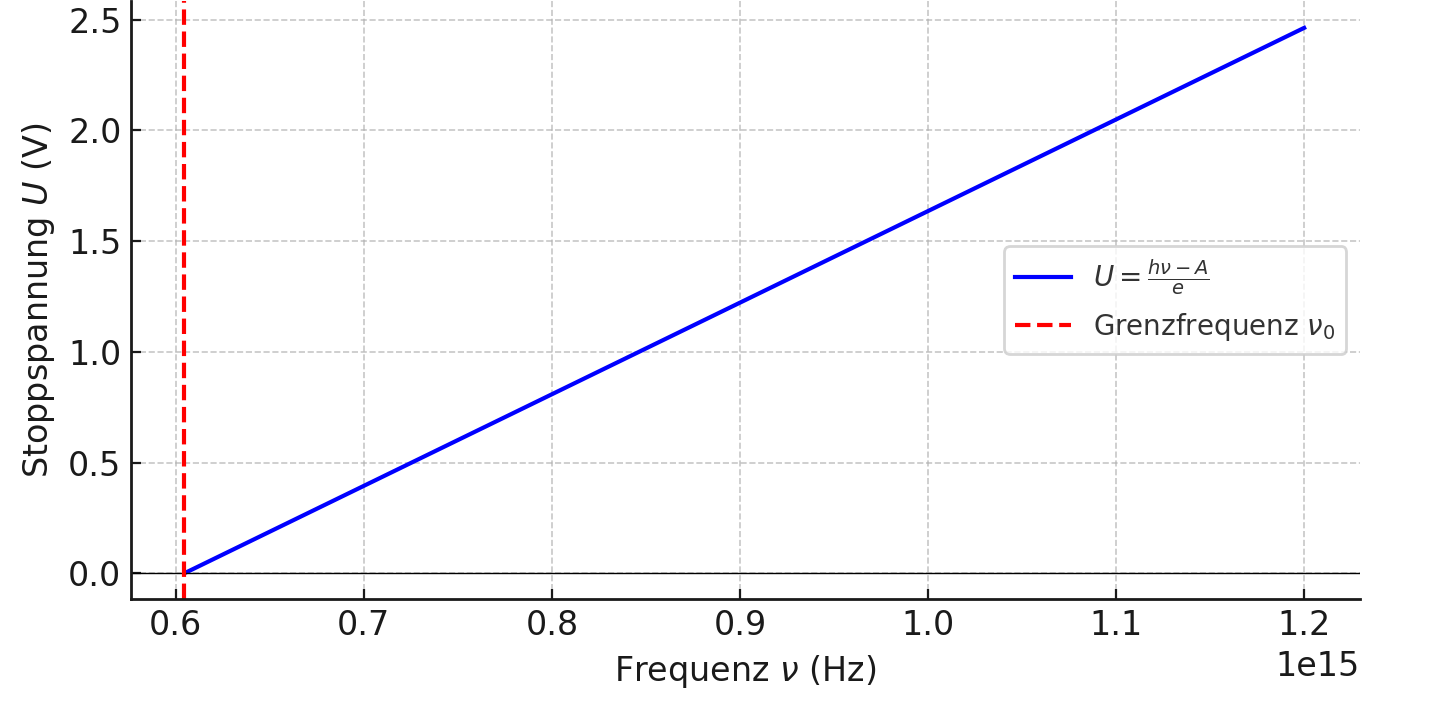
\includegraphics[width=0.65\textwidth]{bilder/photoeffekt.png}
	\caption{lineare Abhängigkeit der Elektronrnernergie}
\end{figure}

\begin{itemize}
	\item Die \textbf{Steigung} der Geraden entspricht \( h/e \)
	\item Der \textbf{x-Achsenabschnitt} \( \nu_0 \) ist die Grenzfrequenz: \( h \nu_0 = A \)\index{Grenzfrequenz}
	\item Für \( \nu < \nu_0 \) tritt keine Emission auf – unabhängig von der Intensität
\end{itemize}

Diese lineare Beziehung wurde von Millikan experimentell mit hoher Genauigkeit bestätigt.\index{Millikan, Robert A.}

\textbf{Dies hat dann zur Folge:}

\begin{quote}
	Die Energie eines Photons hängt allein von der Frequenz ab – nicht von der Lichtintensität.
\end{quote}
\index{Frequenz}\index{Intensität}
\subsubsection{ Vergleich: Wellenmodell vs. Photonenmodell}\index{Wellenmodell}\index{Photonenmodell}\index{Welle-Teilchen-Dualismus@Welle-Teilchen-Dualismus (Kontrast)}

Die Erklärung des Photoeffekts markiert einen tiefgreifenden Paradigmenwechsel in der Physik: von der klassischen Wellenvorstellung des Lichts hin zu einem quantisierten Teilchenbild.\index{Paradigmenwechsel} Um die Tragweite dieses Wechsels zu verdeutlichen, lohnt sich eine direkte Gegenüberstellung beider Modelle.

\vspace{1em}
\begin{table}[H]
	\centering
	\begin{tabular}{|p{4.75cm}|p{4.75cm}|} % vorher 5cm
		\hline
		\textbf{Klassisches Wellenmodell} & \textbf{Photonenmodell (Einstein)} \\
		\hline
		Licht ist eine kontinuierliche Welle im elektromagnetischen Feld & Licht besteht aus einzelnen Quanten (Photonen) mit Energie \( E = h\nu \) \\
		\hline
		Energie wird über die Feldstärke kontinuierlich übertragen & Energie wird stoßartig in diskreten Portionen übertragen \\
		\hline
		Intensität bestimmt die Energieübertragung & Intensität bestimmt nur die \emph{Anzahl} der Photonen, nicht deren Energie \\
		\hline
		Jede Frequenz kann bei genügender Intensität Elektronen lösen & Nur Photonen mit \( h\nu > A \) lösen Elektronen aus \\
		\hline
		Energie wird langsam angesammelt; Zeitverzögerung möglich & Sofortige Emission bei Photontreffer \\
		\hline
	\end{tabular}
	\caption{Vergleich zwischen klassischem Wellenmodell und Photonenmodell beim Photoeffekt}
	\label{tab:vergleich_photoeffekt}
\end{table}
\newpage
\noindent
\vspace{1em}

\begin{tcolorbox}[didaktikbox, title=Didaktische Klarstellung]
	\label{box:didaktischeKlarstellung}
	\small
	Die Intensität des Lichts entscheidet im Wellenmodell über die Stärke der Energieübertragung – im Photonenmodell jedoch nur über die Anzahl der auftreffenden Quanten.\\
	Die Energie eines einzelnen Photons hängt ausschließlich von der Frequenz ab.
\end{tcolorbox}
\vspace{1em}
\index{Intensität}\index{Frequenz}\index{Photon}
\textbf{Typisches Missverständnis:}  
„Helles Licht muss stärkere Elektronen auslösen.“  
$\rightarrow$ \emph{Falsch}, denn bei Licht unterhalb der Grenzfrequenz geschieht – unabhängig von der Helligkeit – gar nichts.\index{Grenzfrequenz}

\textbf{Einordnung:}  
Der Photoeffekt war der erste direkte Nachweis dafür, dass elektromagnetische Strahlung nicht nur Wellencharakter, sondern auch Teilcheneigenschaften besitzt. Diese Dualität wurde später im Konzept des Welle-Teilchen-Dualismus verallgemeinert.\index{Welle-Teilchen-Dualismus}
\subsubsection{Bedeutung für die Physik}\index{Photoeffekt!Bedeutung}\index{Photon}\index{Quantennatur des Lichts@Quantennatur des Lichts}\index{Einstein, Albert}\index{Klassische Elektrodynamik}

Der Photoeffekt war das erste Phänomen, das sich nur durch die Annahme einer diskreten Quantennatur des Lichts erklären ließ. Einsteins Lichtquantenhypothese von 1905 widersprach der klassischen Elektrodynamik und wurde zunächst als spekulativ abgetan. Doch Millikans präzise Bestätigung im Jahr 1916 zwang die Fachwelt, das Bild des Lichts grundlegend zu überdenken.\index{Millikan, Robert A.}

\textbf{Physikalische Konsequenzen:}
\begin{itemize}
	\item Die Energieübertragung des Lichts erfolgt nicht kontinuierlich, sondern in diskreten Quanten – den Photonen.\index{Photon}
	\item Die Energie eines Photons ist proportional zur Frequenz: \( E = h\nu \).\index{Planck-Einstein-Beziehung@$E=h\nu$}\index{Frequenz}
	\item Der Photoeffekt lieferte den ersten direkten experimentellen Nachweis für diese Quantisierung.\index{Photoeffekt!Nachweis}
\end{itemize}

Einstein selbst erhielt 1921 den Nobelpreis – ausdrücklich nicht für die Relativitätstheorie, sondern:\index{Nobelpreis!Einstein 1921}\index{Relativitätstheorie}
\begin{quote}
	„für seine Verdienste um die theoretische Physik, insbesondere für seine Entdeckung des Gesetzes des Photoelektrischen Effekts.“
\end{quote}

Auch Millikan wurde 1923 mit dem Nobelpreis ausgezeichnet – für seine Bestimmung der Elementarladung und seine Arbeiten zum Photoeffekt.\index{Nobelpreis!Millikan 1923}\index{Elementarladung}

\vspace{1em}
\begin{tcolorbox}[hinweisbox, title=Fazit]
	\label{box:fazit der photo}
	\small
	Der Photoeffekt markiert den Anfang des Photonenbegriffs – und damit den Beginn der Quantenphysik.\\
	Er zeigt: Licht besitzt nicht nur Welleneigenschaften, sondern verhält sich unter bestimmten Bedingungen wie ein Teilchen.
\end{tcolorbox}
\index{Quantenphysik}
\vspace{1em}
\textbf{Ausblick:}  
Im nächsten Abschnitt betrachten wir ein weiteres Schlüsselexperiment: die \textbf{Compton-Streuung}. Sie zeigt nicht nur die Energie-, sondern auch die \emph{Impulsübertragung} von Photonen – ein entscheidender Beleg für den Teilchencharakter des Lichts.\index{Compton-Streuung}\index{Impulsübertragung}

\subsection{Die Compton-Streuung}\index{Compton-Streuung}\index{Compton, Arthur H.}\index{Röntgenstrahlung}

\subsubsection{Das Compton-Experiment (1923)}\index{Compton, Arthur H.!Experiment (1923)}

Im Jahr 1923 veröffentlichte der amerikanische Physiker \textbf{Arthur H. Compton} die Ergebnisse eines Streuexperiments mit Röntgenstrahlung, das die Physik revolutionieren sollte. Er ließ hochenergetische Photonen auf nahezu freie Elektronen treffen – etwa in Graphit –, und analysierte die gestreute Strahlung in Abhängigkeit vom Winkel.\index{Elektron}\index{Graphit}

Die zentrale Beobachtung war verblüffend: Das gestreute Licht hatte eine größere Wellenlänge (niedrigere Energie) als das einfallende, und die Wellenlängenverschiebung war systematisch vom Streuwinkel abhängig.\index{Wellenlängenverschiebung}\index{Streuwinkel}

Diese Veränderung ließ sich weder durch klassische Streuung (wie bei Thomson) noch durch Interferenz erklären. Compton interpretierte das Ergebnis als \textbf{elastischen Stoß} zwischen einem Photon und einem Elektron – ganz im Sinne eines Teilchenmodells des Lichts. Damit wurde das Photon nicht nur Träger von Energie, sondern auch von Impuls.\index{Thomson-Streuung}\index{Elastischer Stoß}\index{Photonenimpuls}

\textbf{Physikalisches Prinzip:}
\begin{itemize}
	\item Ein Photon mit Wellenlänge \( \lambda \) trifft auf ein ruhendes Elektron.
	\item Beim Stoß wird das Photon abgelenkt (Streuwinkel \( \theta \)) und gibt dabei Impuls und Energie an das Elektron ab.
	\item Das gestreute Photon besitzt eine neue Wellenlänge \( \lambda' > \lambda \).
\end{itemize}

\textbf{Zentrale Gleichung:}
\[
\Delta \lambda = \lambda' - \lambda = \frac{h}{m_e c}(1 - \cos \theta)
\]\index{Compton-Formel}\index{Compton-Wellenlänge}\index{Elektron!Masse $m_e$}

\vspace{1em}
\begin{figure}[H]
	\begin{center}
		
		
		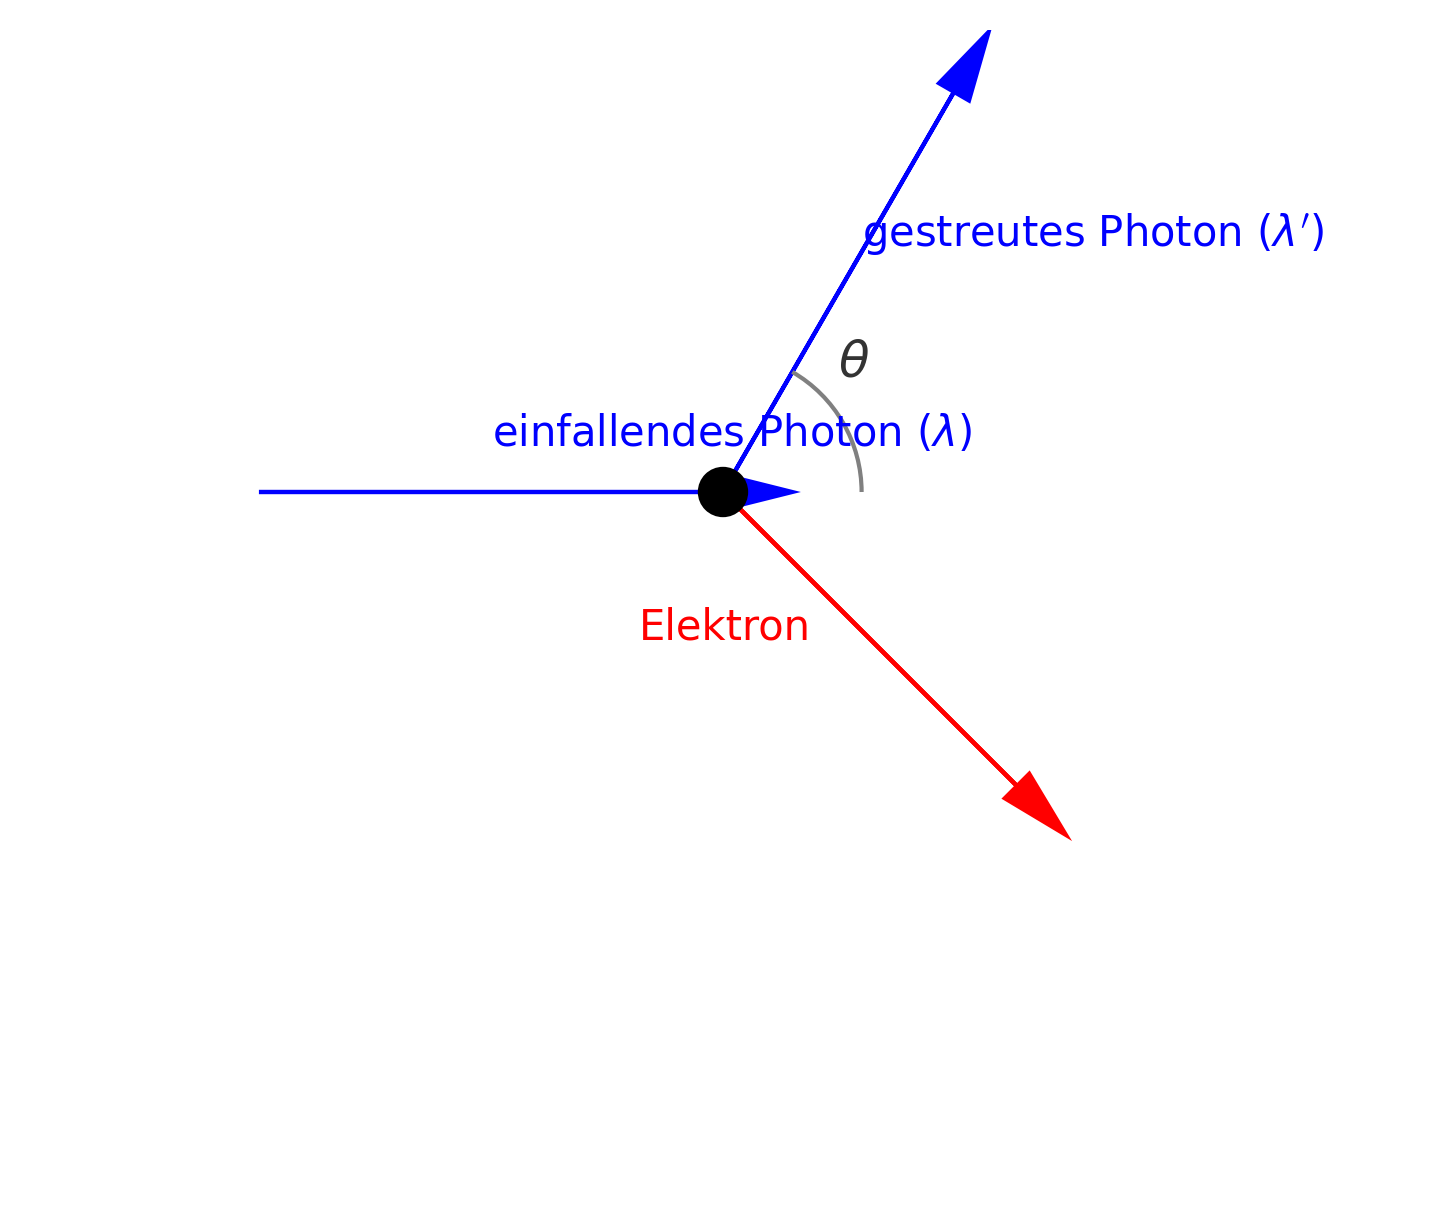
\includegraphics[width=0.6\textwidth]{bilder/compton-schema.png}
	\end{center}
	\caption{Schematische Darstellung der Compton-Streuung: Ein Photon überträgt Impuls auf ein Elektron.}
\end{figure}

\textbf{Bedeutung:}  
Die Compton-Streuung ist der erste experimentelle Beleg dafür, dass Photonen Impuls besitzen – ein entscheidender Schritt zur Anerkennung des Photons als echtes Teilchen. Arthur Compton erhielt dafür 1927 den Nobelpreis für Physik.\index{Photonenimpuls}\index{Nobelpreis!Compton 1927}

\subsubsection{Kompakte Herleitung der Compton-Formel}\index{Compton-Formel!Herleitung}\index{Energieerhaltung}\index{Impulserhaltung}

Die zentrale Beobachtung beim Compton-Effekt ist: Das gestreute Photon hat eine größere Wellenlänge als das einfallende. Diese Verschiebung lässt sich nur erklären, wenn man dem Photon nicht nur Energie \( E = h\nu \), sondern auch Impuls \( p = h/\lambda \) zuschreibt.\index{Planck-Einstein-Beziehung@$E=h\nu$}\index{Photonenimpuls}

\textbf{Grundidee der Herleitung:}
Das Photon trifft auf ein ruhendes Elektron. Beim Stoß wird Energie und Impuls auf das Elektron übertragen. Die Situation ähnelt einem elastischen Stoß zweier Teilchen – mit dem Unterschied, dass eines davon masselos ist.\index{Elastischer Stoß}\index{Masselose Teilchen}
\newpage
\noindent
\textbf{Zentrale Annahmen:}
\begin{itemize}
	\item \textbf{Energieerhaltung:} Die Summe aus Photonenenergie und Elektronenruheenergie bleibt erhalten.
	\item \textbf{Impulserhaltung:} Die Impulsvektoren vor und nach dem Stoß müssen sich vektoriell ausgleichen – in x- und y-Richtung.
	\item \textbf{Photonenimpuls:} Für das Photon gilt \( p = \frac{h}{\lambda} \), für das Elektron relativistische Energie-Impuls-Beziehung.\index{Relativistische Energie-Impuls-Beziehung}
\end{itemize}

Durch Anwendung dieser Erhaltungssätze ergibt sich nach Umformung die \textbf{Compton-Formel}:

\vspace{1em}
\begin{tcolorbox}[mathebox, title=Compton-Formel]
	\label{box:comptonFormel}
	\small
	\[
	\Delta \lambda = \lambda' - \lambda = \frac{h}{m_e c}(1 - \cos \theta)
	\]
\end{tcolorbox}
\vspace{1em}
(Eine ausführlichere Herleitung der Compton-Formel findet sich in Anhang~A, Abschnitt~\ref{anhangA:comptonHerleitung}.) % NEU
\textbf{Physikalische Interpretation:}
\begin{itemize}
	\item Die Wellenlänge des gestreuten Photons ist umso größer, je größer der Streuwinkel \( \theta \) ist.\index{Streuwinkel}
	\item Der Faktor \( \frac{h}{m_e c} \approx 2{,}43 \cdot 10^{-12}\,\mathrm{m} \) wird als \emph{Compton-Wellenlänge} des Elektrons bezeichnet.\index{Compton-Wellenlänge}
	\item Der Effekt zeigt, dass das Photon \emph{Impuls} überträgt – ein klarer Beleg für seinen Teilchencharakter.\index{Photonenimpuls}
\end{itemize}

\vspace{1em}

\subsection{Doppelspaltversuch mit einzelnen Photonen}\index{Doppelspaltversuch}\index{Einzelphoton}\index{Interferenz}\index{Welle-Teilchen-Dualismus}

Ein zentrales Argument für den Wellencharakter des Lichts war seit dem 19. Jahrhundert die Beobachtung von Interferenzmustern – insbesondere im berühmten Doppelspaltversuch. Doch moderne Experimente zeigen: Auch einzelne Photonen, die nacheinander durch den Versuchsaufbau geschickt werden, erzeugen am Schirm ein Interferenzmuster. Dies ist nur erklärbar, wenn man dem Photon auch Wellencharakter zuschreibt.\index{Interferenzmuster}
\newpage
\noindent
\textbf{Experimenteller Aufbau:}
\begin{itemize}
	\item Eine schwache Lichtquelle sendet einzelne Photonen aus – so schwach, dass sich niemals zwei gleichzeitig im Aufbau befinden.\index{Einzelphotonenquelle}
	\item Die Photonen passieren zwei eng beieinanderliegende Spalte (Doppelspalt).\index{Doppelspalt}
	\item Dahinter befindet sich ein lichtempfindlicher Schirm oder Detektor.\index{Detektor}
\end{itemize}

\textbf{Beobachtung:}
\begin{itemize}
	\item Jedes einzelne Photon wird punktuell registriert – wie ein Teilchen.\index{Teilchencharakter des Lichts}
	\item Nach und nach entsteht jedoch ein Interferenzmuster – wie bei einer Welle.\index{Wellencharakter des Lichts}
\end{itemize}

\vspace{1em}
\begin{figure}[H]
	\begin{center}
		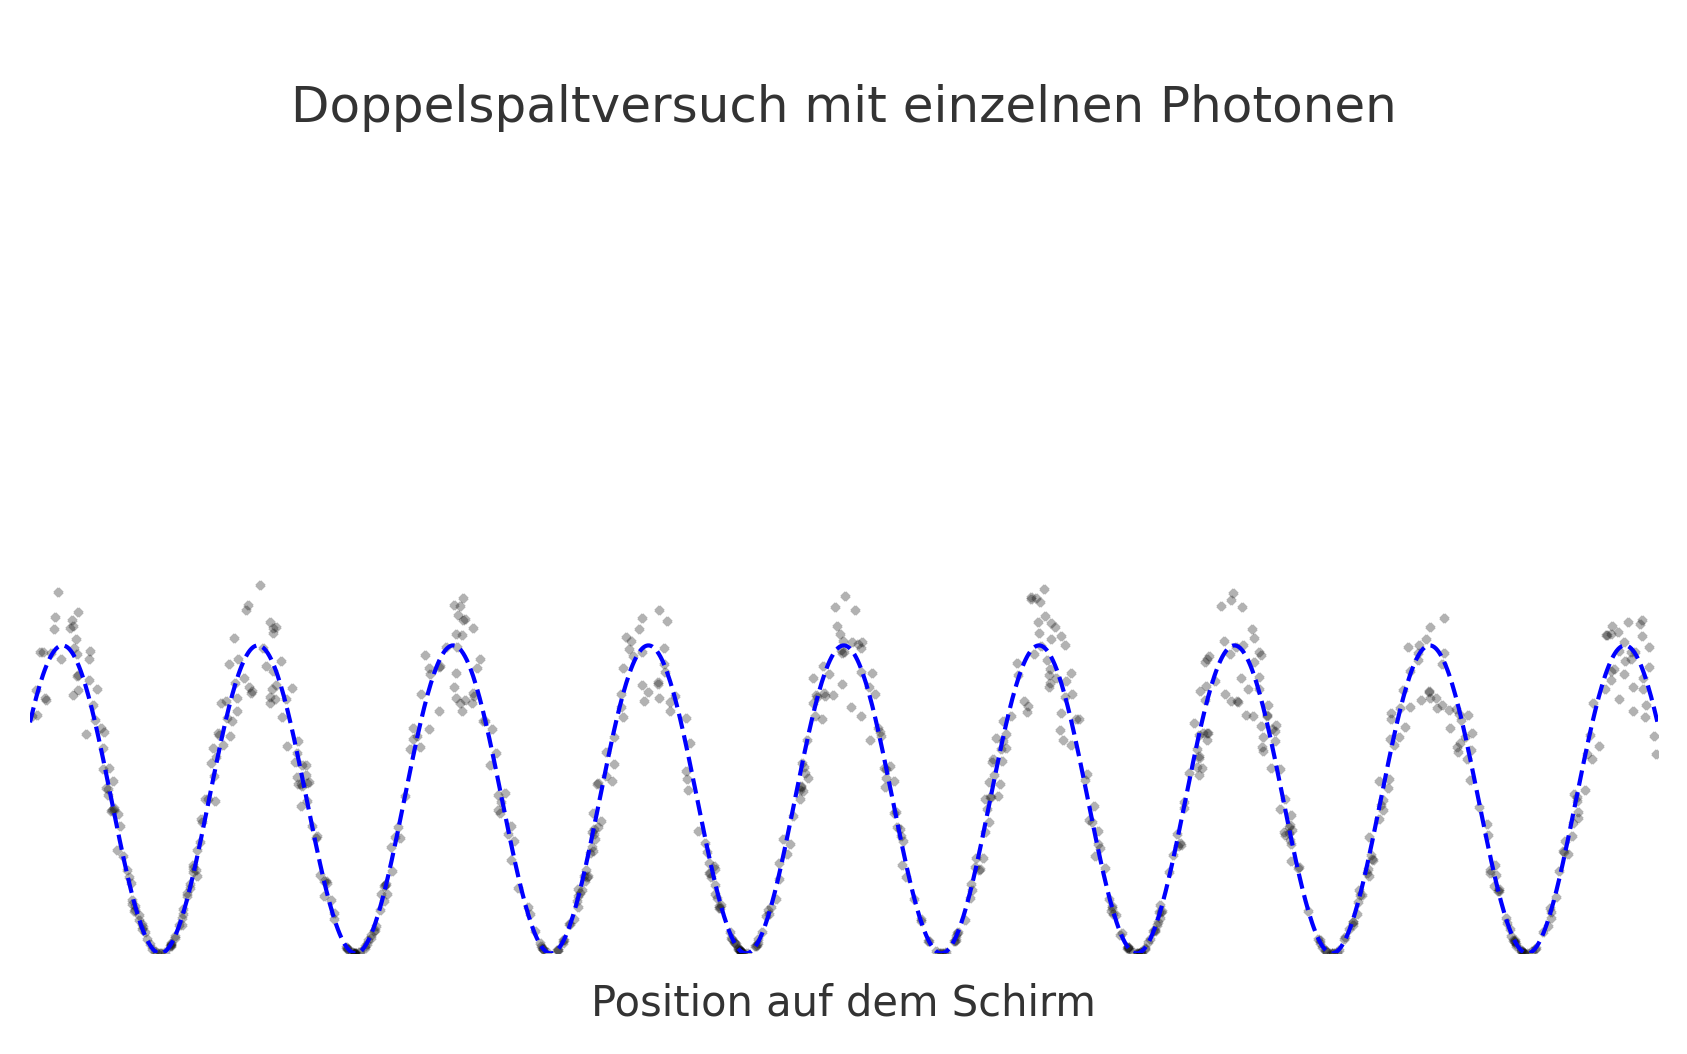
\includegraphics[width=0.65\textwidth]{bilder/doppelspalt-photonen.png}
	\end{center}
	\caption{Doppelspaltversuch mit einzelnen Photonen: Teilchendetektion mit Wellenmuster.}
\end{figure}

\begin{tcolorbox}[physikbox, title=Was die Photonengrafik zeigen soll]
	\label{box:was die photonengrafik}
	\small
	\begin{itemize}
		\item Die Punkte stehen für einzelne Photondetektionen – der Teilchenaspekt des Lichts.
		\item Mit der Zeit entsteht ein Muster, das typisch für Welleninterferenz ist – wie bei Wasserwellen.
		\item Die gestrichelte Linie zeigt nur die statistische Häufigkeit der Auftrefforte – sie ist kein Lichtstrahl und keine reale Welle.
	\end{itemize}
\end{tcolorbox}
\vspace{1em}
(Das mathematische Formalisieren des Doppelspaltversuchs mit einzelnen Photonen und die Superpositionsdarstellung finden sich in Anhang~A, Abschnitt~\ref{anhangA:doppelspalt}.) % NEU
\textbf{Interpretation:}  
Das Photon interferiert offenbar mit sich selbst – es „geht gleichzeitig durch beide Spalte“. Erst beim Nachweis am Schirm kollabiert der Zustand in ein einzelnes Ereignis. Dieses Verhalten lässt sich nur im Rahmen der Quantenmechanik verstehen: Das Photon ist weder klassische Welle noch klassisches Teilchen – es zeigt beides, abhängig vom Experiment.\index{Selbstinterferenz}\index{Quantenmechanik}\index{Zustandskollaps@Kollaps der Wellenfunktion}

\vspace{1em}
\begin{tcolorbox}[hypobox, title=Schlüsselidee]
	\label{box:schlüsselidee}
	\small
	Der Doppelspaltversuch mit einzelnen Photonen zeigt: Die Quantennatur des Lichts beinhaltet sowohl Wellen- als auch Teilcheneigenschaften. Das Interferenzmuster entsteht, obwohl niemals zwei Photonen gleichzeitig im System sind.
\end{tcolorbox}
\vspace{1em}
\begin{tcolorbox}[didaktikbox, title=Wellen-als auch Teilcheneigenschaften]
	\label{box:wellen}
	\small
	Das Interferenzmuster verschwindet sofort, wenn man versucht, den Weg des Photons durch einen der Spalte zu bestimmen. Die Möglichkeit zur Interferenz ist an die \emph{Unkenntnis des Weges} gebunden – ein Grundprinzip der Quantenphysik.
\end{tcolorbox}
\index{Welcher-Weg-Information}

\subsubsection*{Zusammenfassung}\index{Doppelspaltversuch!Zusammenfassung}\index{Superposition}

\phantomsection
\begin{tcolorbox}[didaktikbox, title=Fazit: Ein scheinbar paradoxes Verhalten]
	\label{box:Fazit ein scheinbarer}
	\small
	Selbst wenn Photonen einzeln – also nacheinander – durch den Doppelspalt geschickt werden, entsteht mit der Zeit ein Interferenzmuster.
	
	Das wirft eine tiefgreifende Frage auf: Woher „weiß“ ein einzelnes Photon, dass es Teil eines Musters ist?
	
	Im klassischen Sinne müsste es eine Art Kommunikation zwischen den Photonen geben – doch dem ist nicht so. Jedes Photon scheint mit sich selbst zu interferieren. Die Quantenmechanik erklärt dies durch die \textbf{Überlagerung aller möglichen Wege}: Das Photon ist nicht durch den einen oder den anderen Spalt gegangen – sondern durch beide, solange der Weg nicht gemessen wird.
	
	Diese Vorstellung widerspricht unserer Alltagserfahrung – ist aber experimentell zweifelsfrei belegt. Der Doppelspaltversuch ist damit ein Schlüsselergebnis der Quantenphysik.
	
	Der Doppelspaltversuch mit einzelnen Photonen stellt unser klassisches Denken infrage:  
	Wie kann ein einzelnes Photon zum Aufbau eines Interferenzmusters beitragen, obwohl kein zweites Photon gleichzeitig im Versuchsaufbau ist?
	
	Offenbar scheint jedes Photon mit sich selbst zu interferieren. In der Sprache der Quantenmechanik bedeutet das: Solange kein Messgerät den Weg bestimmt, überlagern sich alle möglichen Wege gleichzeitig – auch „durch beide Spalte zugleich“.
	
	Diese Superposition kollabiert erst bei der Detektion zu einem einzelnen Punkt. Das Interferenzmuster entsteht nicht durch Wechselwirkung der Photonen untereinander, sondern durch die \emph{Statistik vieler Einzelmessungen} – und durch die quantenmechanische Struktur des Zustandsraums.
	
	Was nach „Kommunikation“ aussieht, ist in Wahrheit ein Ausdruck der Nichtklassizität der Quantenwelt.
\end{tcolorbox}

\subsection{Antibunching: Der Nachweis einzelner \newline Photonen}\index{Antibunching}\index{Einzelphoton}\index{Einzelphotonenquelle}\index{Strahlteiler}\index{Detektor}

Ein besonders überzeugender experimenteller Beweis für die Existenz einzelner Photonen liefert das Phänomen des \textbf{Antibunching}. Dabei wird eine Lichtquelle verwendet, die nur jeweils ein Photon auf einmal abstrahlen kann – z.\,B. ein fluoreszierendes Atom oder Quantenpunkt.\index{Quantenpunkt}\index{Fluoreszenz}

In einem Aufbau mit Strahlteiler und zwei Detektoren zeigt sich: Es \emph{kommt niemals vor}, dass beide Detektoren gleichzeitig ein Signal registrieren. Das bedeutet: Es gibt kein „halbes“ Photon – sondern immer genau eines, das entweder hier oder dort ankommt.\\
\textbf{Warum widerspricht das der klassischen Wellenvorstellung?} \\
In der klassischen Theorie ist Licht eine kontinuierliche elektromagnetische Welle. Trifft eine solche Welle auf einen Strahlteiler, so wird sie \emph{aufgeteilt}: Ein Teil geht nach links, der andere nach rechts. Damit müssten – zumindest bei starker Intensität – auch beide Detektoren gleichzeitig ein Signal registrieren.\index{Klassische Elektrodynamik}\index{Wellenmodell}

Beim Antibunching hingegen zeigt sich: \emph{Nie} werden beide Detektoren gleichzeitig ausgelöst. Das bedeutet, dass das Licht nicht aufgeteilt ankommt, sondern in \textbf{unteilbaren Energiepaketen} – einzelnen Photonen. Genau das widerspricht der Vorstellung einer klassischen Welle.\index{Photon!Unteilbarkeit}

\vspace{1em}
\begin{tcolorbox}[physikbox, title=Was Antibunching zeigt]
	\label{box:wasAntibunching}
	\small
	Licht kann nicht gleichzeitig in zwei Richtungen aufgeteilt werden, wenn es aus einzelnen Photonen besteht.\\
	Dies widerspricht jeder klassischen Wellenvorstellung – aber entspricht genau dem Verhalten unteilbarer Lichtquanten.
\end{tcolorbox}
\vspace{1em}
(Eine mathematische Beschreibung der zweiten Ordnungs-Korrelations\-funktion \( g^{(2)}(0) \) findet sich in Anhang~A, Abschnitt~\ref{anhangA:antibunching}.) % NEU
\subsection{Hong-Ou-Mandel-Effekt: \newline Interferenz zweier Photonen}\index{Hong-Ou-Mandel-Effekt}\index{Ununterscheidbarkeit (Photonen)@Ununterscheidbarkeit von Photonen}\index{Wahrscheinlichkeitsamplitude}\index{Strahlteiler}

Ein weiteres eindrucksvolles Experiment ist der \textbf{Hong-Ou-Mandel-Effekt}. Zwei identische Photonen werden aus zwei entgegengesetzten Richtungen auf einen halbdurchlässigen Spiegel (Strahlteiler) gelenkt.
\begin{figure}[H]
	\begin{center}
		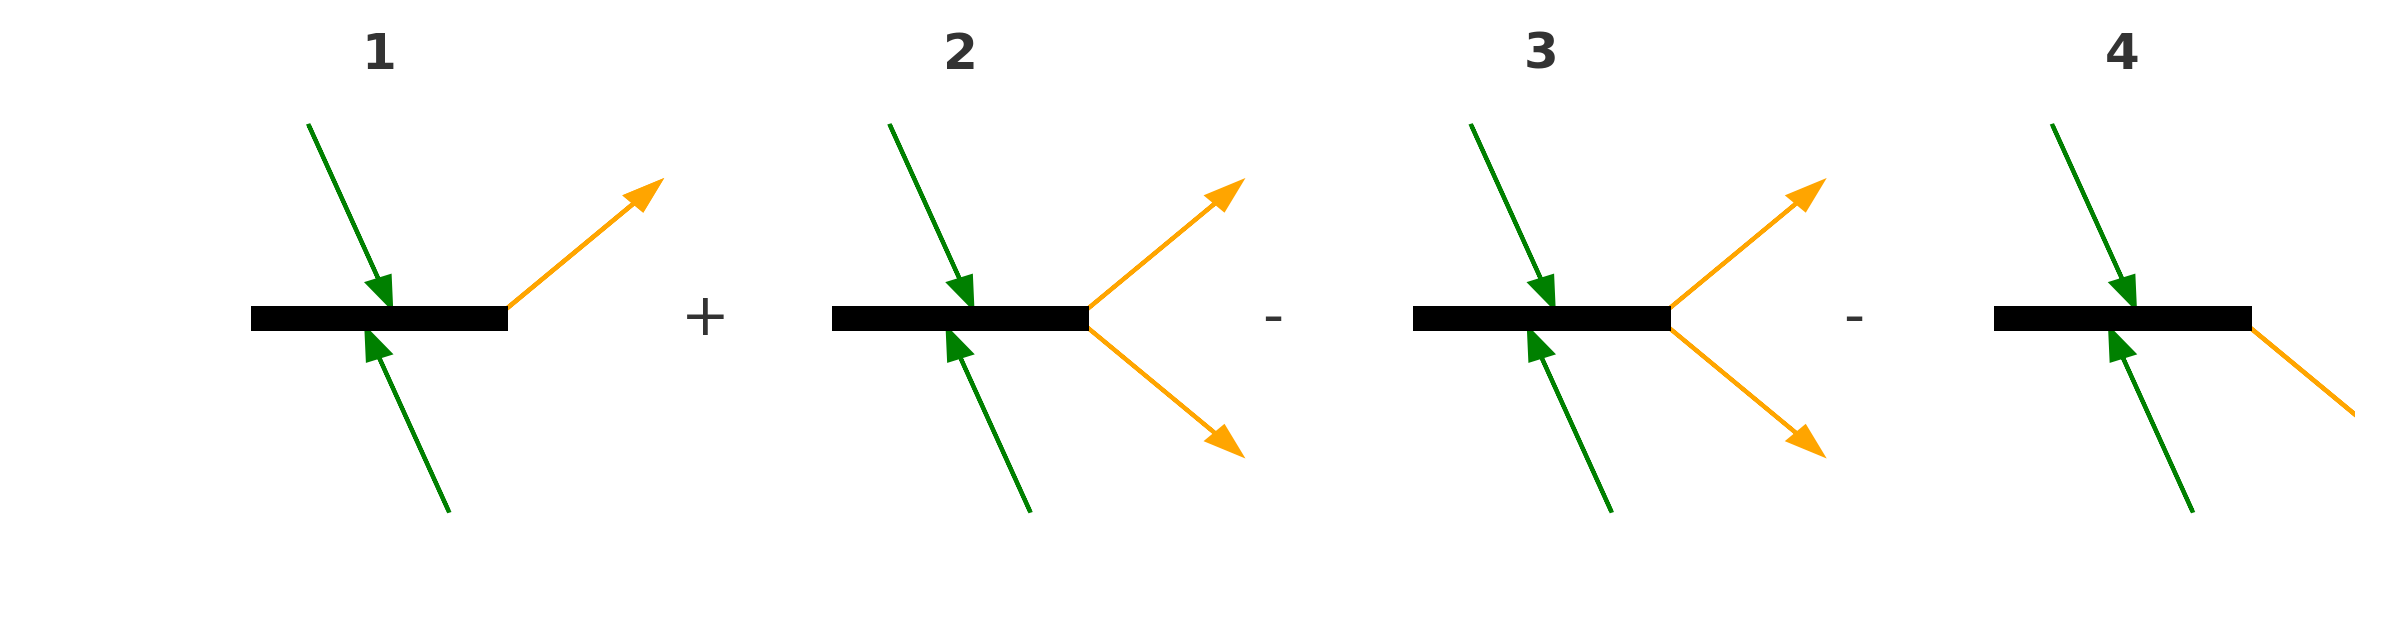
\includegraphics[width=0.95\textwidth]{bilder/hom_interferenzpfade_korrigiert.png}
		
	\end{center}
	\caption{Vier mögliche Pfade zweier Photonen am Strahlteiler.\\
		Die mittleren Fälle führen zu Koinzidenz – löschen sich aber durch Interferenz aus}
\end{figure}

\begin{tcolorbox}[hinweisbox, title=Was diese Darstellung zeigt]
	\label{box:was diese Darstellun}
	\small
	Das Diagramm zeigt die vier möglichen Pfade, die zwei identische Photonen beim Auftreffen auf einen Strahlteiler nehmen können.\\
	In den Fällen 1 und 4 verlassen beide Photonen gemeinsam denselben Ausgang – wie es experimentell beobachtet wird.
	
	Die Pfade 2 und 3 würden dazu führen, dass die Photonen an unterschiedlichen Detektoren ankommen (Koinzidenz). Doch genau diese Fälle löschen sich durch destruktive Interferenz aus – aufgrund der Ununterscheidbarkeit der Photonen und der quantenmechanischen Überlagerung ihrer Amplituden.
	
	Das Ergebnis: Bei perfekter Überlappung werden niemals gleichzeitig beide Detektoren ausgelöst – ein klarer Hinweis auf die Quantennatur des Lichts.
\end{tcolorbox}

Nach klassischer Erwartung müsste jedes Photon mit 50\,\% Wahrscheinlichkeit reflektiert oder transmittiert werden. Doch in der Quantenrealität passiert etwas anderes: Beide Photonen verlassen immer denselben Ausgang – nie gegensätzlich.\index{Reflexion}\index{Transmission}

Dieses Phänomen entsteht durch die Interferenz der \emph{Wahrscheinlichkeitsamplituden} beider Prozesse. Es zeigt: Photonen sind ununterscheidbar und können auf Quantenebene interferieren – nicht als Felder, sondern als Teilchen mit Wellennatur.\index{Interferenz}\index{Ununterscheidbarkeit (Photonen)@Ununterscheidbarkeit von Photonen}

\vspace{1em}
\begin{tcolorbox}[physikbox, title=Was der HOM-Effekt zeigt]
	\label{box:HOM-Effekt}
	\small
	Zwei Photonen können „verhindern“, dass sie unterschiedliche Wege nehmen – durch Interferenz ihrer Quantenzustände.\\
	Dies ist nur erklärbar, wenn man Photonen als ununterscheidbare Quantenteilchen betrachtet.
\end{tcolorbox}

\subsection{Fazit}\index{Photoeffekt}\index{Compton-Streuung}\index{Doppelspaltversuch}\index{Antibunching}\index{Hong-Ou-Mandel-Effekt}\index{Welle-Teilchen-Dualismus}

\begin{tcolorbox}[hinweisbox, title=Was die Experimente über Licht zeigen]
	\label{box:was die Experimente}
	\small
	Die vier in diesem Kapitel behandelten Experimente – Photoeffekt, Compton-Streuung, Doppelspalt mit einzelnen Photonen und moderne Quantenexperimente wie Antibunching und Hong-Ou-Mandel-Effekt – zeigen eindrucksvoll, dass Licht nicht allein durch klassische Modelle erklärbar ist.
	
	\begin{itemize}
		\item Der \textbf{Photoeffekt} zeigt: Licht überträgt \emph{Energie} in diskreten Portionen (Photonen).
		\item Die \textbf{Compton-Streuung} zeigt: Photonen besitzen auch \emph{Impuls} – wie Teilchen.
		\item Der \textbf{Doppelspaltversuch} zeigt: Photonen zeigen \emph{Wellenmuster} in ihrer Verteilung – selbst wenn sie einzeln auftreten.
		\item \textbf{Antibunching} und der \textbf{Hong-Ou-Mandel-Effekt} zeigen: Photonen sind \emph{nicht teilbar}, \emph{nicht klassisch unterscheidbar} und unterliegen den Regeln der Quantenmechanik.
	\end{itemize}
	(Eine detailliertere Herleitung der quantenmechanischen Interferenz am Strahlteiler beim HOM-Effekt findet sich in Anhang~A, Abschnitt~\ref{anhangA:HOM}.) % NEU
	Diese Experimente beweisen gemeinsam: Licht ist kein Entweder-Oder aus Welle und Teilchen – es ist beides zugleich, abhängig vom Experiment. Der Photonenbegriff ist damit nicht nur ein Rechenkonzept – sondern physikalisch real.
\end{tcolorbox}
